\documentclass{article}
%Gummi|065|=)
\usepackage{graphicx}
\title{\textbf{Practica 2}}
\author{Omar Errandi}
\date{}
\begin{document}

\maketitle

\section{Consider the language over the alphabet \{a, b\} that only contains the string \emph a.
}
\textbf a - Build a DFA that recognizes this language and rejects all those strings that
do not belong to the language.
\\

Primero de todo planteamos  el enunciado y deducimos como va a ser el DFA. 
El lenguaje que reconoce es:

L(G) = a

Se trata de un ejercicio sencillo. Tenemos tres automatas, el inicial ($q_0$) transita al final($q_1$) si la cadena consumida es a; si es b transita al tercer estado. En el tercer estado($q_2$)  habra un bucle reflexivo de la cadena b y a. En el estado final, si  hay alguna cadena restante, sea a o b,  transita al tercer estado.
  Dada la gramatica G =  $(\{q_0,  q_1, q_2\}, \{a, b\}, \delta, q_0, \{q_1\})$.
  
  Definimos la funcion de transicion $\delta$:
  
  $\delta (q_0, a) =  q_1$
  
  $\delta (q_0, b) =  q_2$
  
  $\delta (q_1, a) =  q_2$
  
  $\delta (q_1, b) =  q_2$
  
  $\delta (q_2, a) =  q_2$
  
  $\delta (q_2, b) =  q_2$
  
  
  Una vez definido  todo, pasamos a diseñarlo en JFLAP.
  
  	\centering
	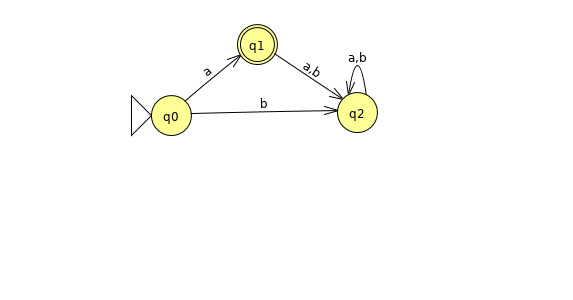
\includegraphics[scale=0.53]{DFA_P2}
	\flushleft
	
\textbf b  - Test the automaton that you have created by introducing 6 chains.
	
	Una vez diseñado el DFA testeamos con diferentes cadenas la  aceptacion y el rechazo de cadenas que no son la cadena "a".
  
  \centering
	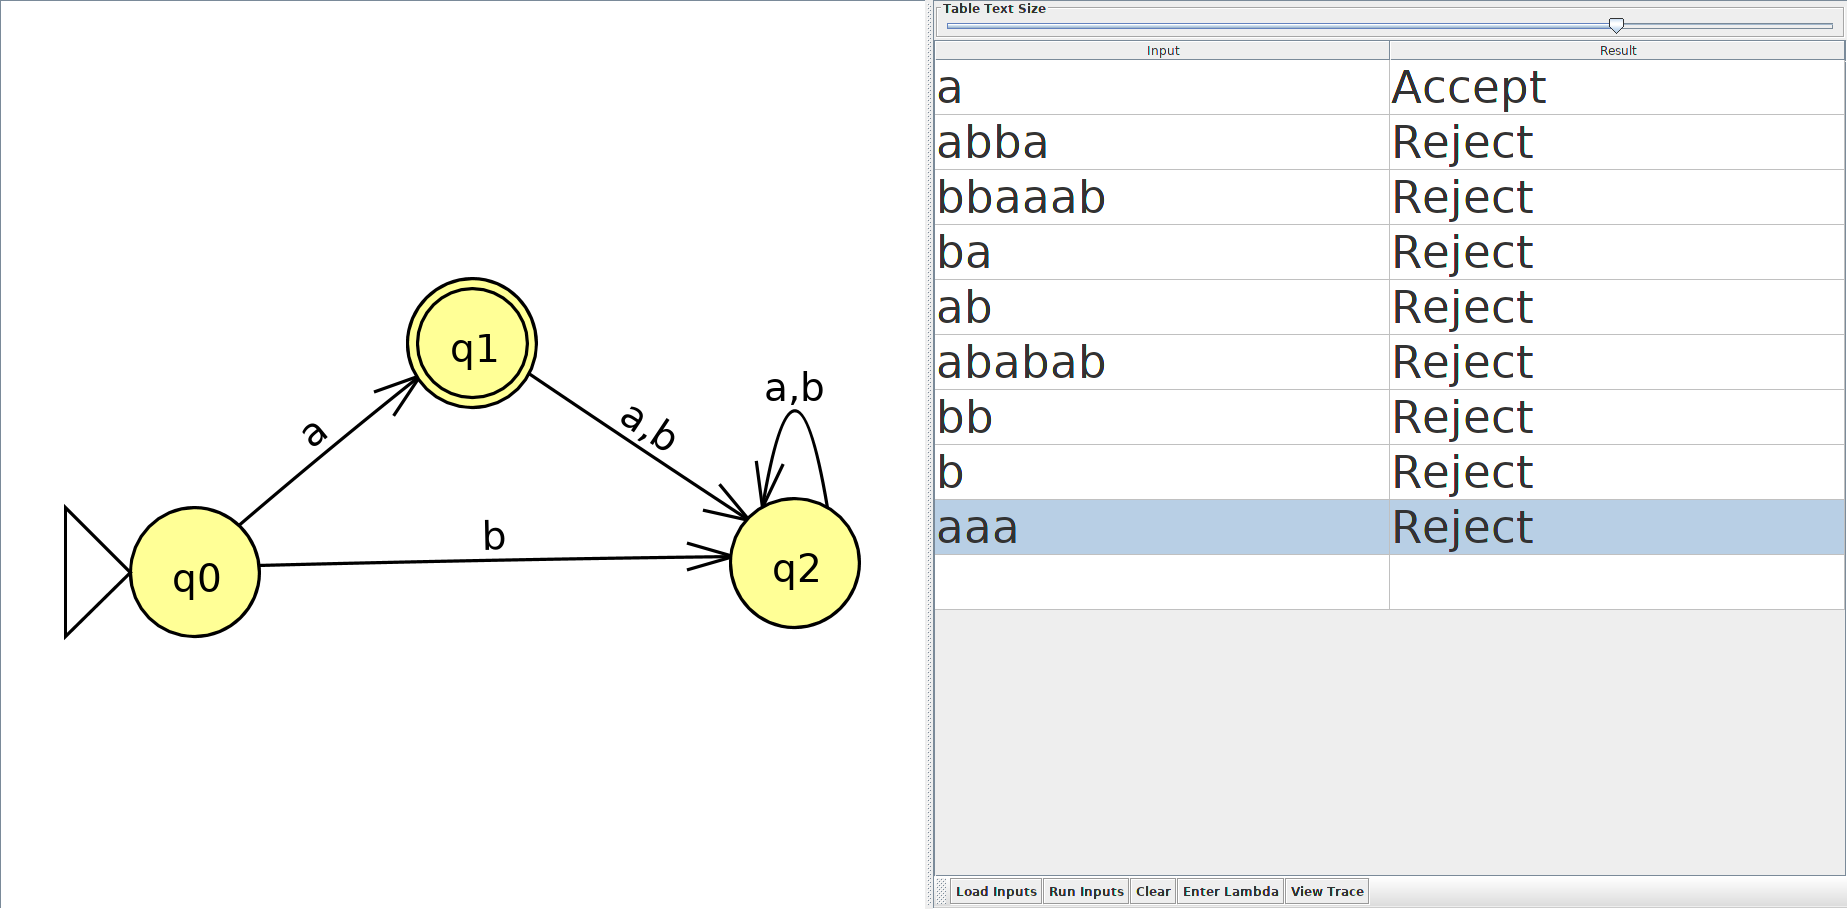
\includegraphics[scale=0.15]{DFA_P2_conTabla}
	
	
	
	

\flushleft
	















\section{Finite automaton in Octave:}

\textbf a. Open the Octave finiteautomata.m script and test it with the given example (see script help) in the GitHub repository.

En el documento de git vienen ya automatas predefinidos, por lo tanto elegire uno al azar y lo probare.
En este caso elijo el automata aa*bb*.
En el Octave ejecutamos:

\centering
finiteautomata("aa*bb*", "ab", "LaTeX")
\flushleft

$M = ( {q_0, q_1, q_2}, {a, b}, q_0, {q_2}, {(q_0, a, q_1), (q_1, a, q_1), (q_1, b, q_2), (q_2, b, q_2)} )$

$w = ab$

$(q_0, ab) \vdash (q_1, b) \vdash (q_2, \varepsilon)$

x $\in$ L(M)


\textbf b. Specify in finiteautomata.json the  automaton created in Activity 1 and test it with the script!

Siguiendo el  ejemplo ya hecho en "finiteautomata.json", en este mismo creamos otro automata llamado DFA\_a con su gramatica correspondiente.

\{
    "name" : "DFA\_a",
    
    "representation" : \{
    
      "K" : ["q0", "q1", "q2"],
      
      "A" : ["a", "b"],
      
      "s" : "q0",
      
      "F" : ["q1"],
      
      "t" : [["q0", "a", "q1"],
             ["q0", "b", "q2"],
             ["q1", "a", "q2"],
             ["q1", "b", "q2"],
	     ["q2", "a", "q2"],
             ["q2", "b", "q2"]]
             
      \}
      
  \}
  
  
Una vez definido el automata del primer ejercico, ejecutamos en octave dicho modelo con la cadena \emph w = a:


	\centering
	$finiteautomata("DFA\_a", "a", "LaTeX")$
	\flushleft
El resultado que nos genera Octave es:

$M = ( {q_0, q_1, q_2}, {a, b}, q_0, {q_1}, {(q_0, a, q_1), (q_0, b, q_2), (q_1, a, q_2), (q_1, b, q_2), (q_2, a, q_2), (q_2, b, q_2)} )$

$w = a$

$(q_0, a) \vdash (q_1, \varepsilon)$

\emph x $\in$ L(M)



Concluimos con que nuestro automata funciona correctamente.



\end{document}
